% !TeX spellcheck = en_US
\chapter{Imitation Learning}

\ac{IL}, \ac{aka} \textit{Behavior Cloning}, \ac{LfD}, essentially, this is \hlb{\underline{supervised learning}}. One problem might arise: applying the learned policy $\pi_{\theta}$ might lead to different action $\textbf{a}_t$, which then leads to different observations and states, comparing to the given dataset: $p_{data}(\textbf{o}_t)~\neq~p_{\pi_{\theta}}(\textbf{o}_t)$. This \hlb{distribution mismatch} can be tackled by adding on-policy data.

\section{DAgger}
\label{sec:dagger}
\ac{dagger} aggregates training data from $p_{\pi_{\theta}}(\textbf{o}_t)$ instead of just $p_{data}(\textbf{o}_t)$. Without \ac{dagger}, it is proven that the error will grow quadratically with the number of time steps $\mathcal{O}(\epsilon T^2)$. \cite{ross2011ais}
\begin{enumerate}
	\item \tikzmark{il1}Train $p_{\pi_{\theta}}(\textbf{o}_t)$ from human data $\mathcal{D} = \{ (\textbf{o}_t, \textbf{a}_t)_i\}$
	\item Run $p_{\pi_{\theta}}(\textbf{o}_t)$ to get data set $\mathcal{D}_\pi = \{\textbf{o}_1, \dots, \textbf{o}_M\}$
	\item Ask human to label $\mathcal{D}_\pi$ with action $\textbf{a}_t$
	\item \tikzmark{il4}Aggregate $\mathcal{D} \leftarrow \mathcal{D} \bigcup \mathcal{D}_\pi$
	\begin{tikzpicture}[overlay,remember picture]
		\draw[very thick, -latex] ([xshift=-7mm,yshift=1mm]pic cs:il4) --++ (-.5,0) |- ([xshift=-7mm,yshift=1mm]pic cs:il1);
	\end{tikzpicture}
\end{enumerate}
The major problem with \ac{dagger} is that it requires human input again in step 3.

\subsection{Recap}
\begin{itemize}
	\item Requires human to annotate the data
	\item Often (but not always) insufficient by itself (distribution mismatch problem)
	\item Sometimes works well
\end{itemize}
\hlb{Problems:}
\begin{itemize}
	\item Non-Markovian behavior
	\item Multimodal behavior
\end{itemize}
\hlb{Solutions:}
\begin{itemize}
	\item Output a mixture of Gaussians
	\item Latent variable models
	\item Auto-regressive discretization (\href{https://www.youtube.com/watch?v=988gLurg01U&list=PL_iWQOsE6TfURIIhCrlt-wj9ByIVpbfGc&index=7}{src})
\end{itemize}

\section{Visual Imitation Learning}
\subsection{Problem Formulation}
\hlb{Problem setting:} given third-person-view images, output sequence of agent actions.
\begin{align}
	O_{human} &= \{ o_{h,0}, o_{h,1}, \dots, o_{h,T} \} && \text{Input: sequence of visual observations}\\
	A_{robot} &= \{ a_{r,0}, a_{r,1}, \dots, a_{r,T} \} && \text{Output: sequence of agent actions}
\end{align}

\subsection{Data Collection}

\begin{itemize}
	\item Kinesthetic teaching: tedious, time consuming labor work. \cite{tykal2016incrementally}
	\item Human teleoperation: expensive and/or complex, but possibly with large amount of rich and scalable data \cite{zhang2018deep}
	\item Demonstration using assistive tools: is simple but works with one specific \ac{ee} at a time \cite{young2020visual}
\end{itemize}

\begin{figure}[hbt!]
	\centering
	\begin{subfigure}[b]{0.25\textwidth}
		\centering
		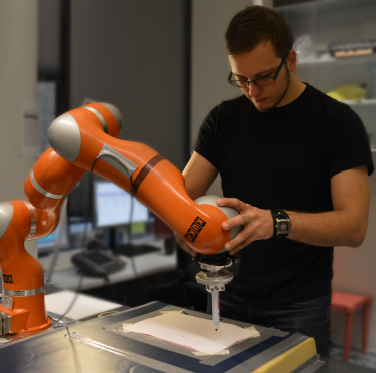
\includegraphics[width=\textwidth]{kinesthetic-teaching.png}
		\caption{Kinesthetic teaching. \cite{tykal2016incrementally}}
	\end{subfigure}
	\hfill
	\begin{subfigure}[b]{0.4\textwidth}
		\centering
		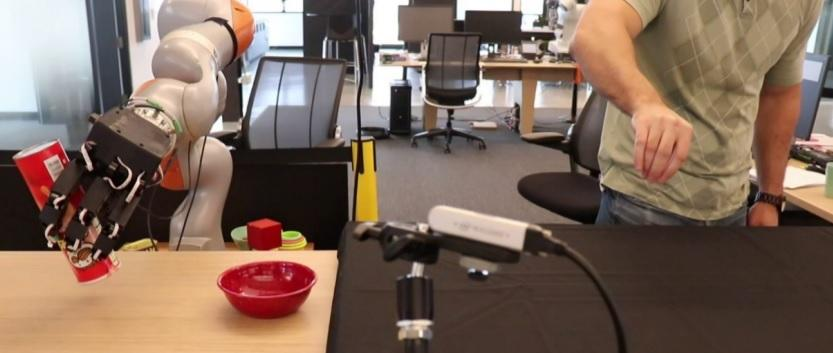
\includegraphics[width=\textwidth]{dexpilot.png}
		\caption{Human teleoperation. \cite{handa2020dexpilot}}
	\end{subfigure}
	\hfill
	\begin{subfigure}[b]{0.3\textwidth}
		\centering
		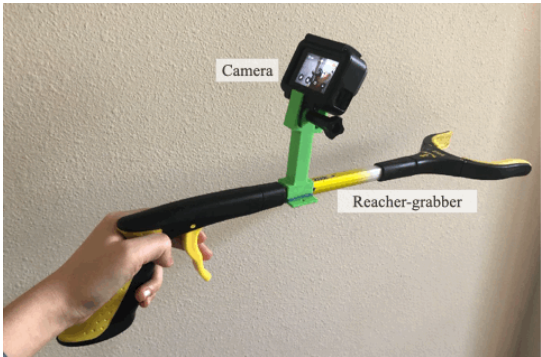
\includegraphics[width=\textwidth]{demoat.png}
		\caption{Assistive tools. \cite{young2020visual}}
	\end{subfigure}
	\caption{Different data collection approaches for visual imitation learning.}
\end{figure}

\subsection{Third Person Visual Imitation}
\citeaustitle{sharma2019third}
\begin{itemize}
	\item The high-level sub-goal generator $ f_{H} $: produces sequence of images, as visual sub-goals, from the images of expert demonstrations
	\begin{align}
		&f_{H}: \mathcal{O}_{rob} \times \mathcal{O}_{h} \times \mathcal{O}_{h} \rightarrow \mathcal{O}_{rob} && \begin{matrix*}[l]
			&\mathcal{O}_{rob} &- \text{robot observation space}\\
			&\mathcal{O}_{h} &- \text{human observation space}
		\end{matrix*}\\
		&f_{H}(o_{r,t}, o_{h,t}, o_{h,t+k}) = o_{r,t+k} && \begin{matrix*}[l]
			&o_{r,t} &- \text{robot observation at time $t$}\\
			&o_{h,t} &- \text{human observation at time $t$}
		\end{matrix*}
	\end{align}
	\item The low-level controller $ \pi_{L} $: produces action plans from the visual sub-goals
	\begin{align}
		&\pi_{L}: \mathcal{O}_{rob} \times \mathcal{O}_{rob} \rightarrow \mathcal{A}_{rob} && \begin{matrix*}[l]
			&\mathcal{O}_{rob} &- \text{robot observation space}\\
			&\mathcal{A}_{rob} &- \text{robot action space}
		\end{matrix*}\\
		&\pi_{L}(o_{r,t}, o_{r,t+k}) = a_{r,t} && \begin{matrix*}[l]
			&o_{r,t} &- \text{robot observation at time $t$}\\
			&a_{r,t} &- \text{robot action at time $t$}
		\end{matrix*}
	\end{align}
\end{itemize}

\hlb{Limitations:} All limitations are probably due to the fact that the authors tried to formulate their goal-generator using the image-to-image translation model \texttt{pix2pix} (\href{https://github.com/pathak22/hierarchical-imitation}{\texttt{github repo}}).
\begin{itemize}
	\item The view points for third-person-view and the robot's first-person-view are \hlr{fixed}.
	\item Even comparing to pix2pix, they have a very strange formulation (personal opinion)
	\item Generate \hlr{low-quality} goal images
	\item Tried, then use \hlr{"bad"} loss functions ($ \mathcal{L}1, \mathcal{L}2 $ loss, \ac{SSIM})
	\item Both high-level and low-level controllers required \hlr{kinesthetic} data collection.
	\item It might also be simpler using optical flow.
	\item Unclear about the baselines comparisons?? 
\end{itemize}

\subsection{One-Shot Visual Imitation Learning with Meta-learning}
\todo{??} \citeaustitle{finn2017one}

\subsection{Others}
There are many works on robotic visual imitation learning. This subsection summarizes their ideas.
\begin{itemize}
	\item Improving generalization with:
	\begin{itemize}
		\item Transformer / Attention network \cite{dasari2020transformers}
		\item Domain randomization \cite{zhou2021manipulator}
		\item Multi-task, instead of one task with many variations \cite{mandi2022towards}
	\end{itemize}
\end{itemize}

\subsection{Proposal}
Perhaps the only way to be able to work with diverse view points and diverse \ac{ee} tools is to formulate interactions with a graph, and with a library of motor primitives for that specific \ac{ee}.

\subsection{References}
\begin{itemize}
	\item \citeaustitle{finn2017one}
	\item \citeaustitle{handa2020dexpilot}
\end{itemize}
